\documentclass{wissdoc}
% Autor: Roland Bless 1996-2009, bless <at> kit.edu
% ----------------------------------------------------------------
% Diplomarbeit - Hauptdokument
% ----------------------------------------------------------------
%%
%% $Id: diplarb.tex 53 2009-12-10 12:23:37Z bless $
%%
% wissdoc Optionen: draft, relaxed, pdf --> siehe wissdoc.cls
% ------------------------------------------------------------------
% Weitere packages: (Dokumentation dazu durch "latex <package>.dtx")
\usepackage{bibgerm}
\usepackage[numbers,sort&compress]{natbib}
% \usepackage{varioref}
% \usepackage{verbatim}
% \usepackage{float}    %z.B. \floatstyle{ruled}\restylefloat{figure}
% \usepackage{subfigure}
% \usepackage{fancybox} % f�r schattierte,ovale Boxen etc.
% \usepackage{tabularx} % automatische Spaltenbreite
% \usepackage{supertab} % mehrseitige Tabellen
% \usepackage[svnon,svnfoot]{svnver} % SVN Versionsinformation 
%% ---------------- end of usepackages -------------

%\svnversion{$Id: diplarb.tex 53 2009-12-10 12:23:37Z bless $} % In case that you want to include version information in the footer

%% Informationen f�r die PDF-Datei
\hypersetup{
 pdfauthor={N.N.},
 pdftitle={Not set}
 pdfsubject={Not set},
 pdfkeywords={Not set}
}

% Macros, nicht unbedingt notwendig
%%%%%%%%%%%%%%%%%%%%%%%%%%%%%%%%%%%%%%%%%%%%%%%%%%%%%%%%%%
% macros.tex -- einige mehr oder weniger nuetzliche Makros
% Autor: Roland Bless 1998
%%%%%%%%%%%%%%%%%%%%%%%%%%%%%%%%%%%%%%%%%%%%%%%%%%%%%%%%%%
% $Id: macros.tex 33 2007-01-23 09:00:59Z bless $
%%%%%%%%%%%%%%%%%%%%%%%%%%%%%%%%%%%%%%%%%%%%%%%%%%%%%%%%%%


%%%%%%%%%%%%%%%%%%%%%%%
% Kommentare 
%%%%%%%%%%%%%%%%%%%%%%%
\ifnotdraftelse{
\newcommand{\Kommentar}[1]{}
}{\newcommand{\Kommentar}[1]{{\em #1}}}
% Alles innerhalb von \Hide{} oder \ignore{} 
% wird von LaTeX komplett ignoriert (wie ein Kommentar)
\newcommand{\Hide}[1]{}
\let\ignore\Hide

%%%%%%%%%%%%%%%%%%%%%%%%%
% Leere Seite ohne Seitennummer, wird aber gezaehlt
%%%%%%%%%%%%%%%%%%%%%%%%%

\newcommand{\leereseite}{% Leerseite ohne Seitennummer, n�chste Seite rechts (wenn 2-seitig)
 \clearpage{\pagestyle{empty}\cleardoublepage}
}
%%%%%%%%%%%%%%%%%%%%%%%%%%
% Flattersatz rechts und Silbentrennung, Leerraum nach rechts maximal 1cm
%%%%%%%%%%%%%%%%%%%%%%%%%%
\makeatletter
\newcommand{\myraggedright}{%
 \let\\\@centercr\@rightskip 0pt plus 1cm
 \rightskip\@rightskip
  \leftskip\z@skip
  \parindent\z@
  \spaceskip=.3333em
  \xspaceskip=.5em}
\makeatother

\makeatletter
\newcommand{\mynewline}{%
 \@centercr\@rightskip 0pt plus 1cm
}
\makeatother


%%%%%%%%%%%%%%%%%%%%%%%%%%
% F�r Index
%%%%%%%%%%%%%%%%%%%%%%%%%%
\makeatletter
\def\mydotfill{\leavevmode\xleaders\hb@xt@ .44em{\hss.\hss}\hfill\kern\z@}
\makeatother
\def\bold#1{{\bfseries #1}}
\newbox\dbox \setbox\dbox=\hbox to .4em{\hss.\hss} % dot box for leaders
\newskip\rrskipb \rrskipb=.5em plus3em % ragged right space before break
\newskip\rrskipa \rrskipa=-.17em plus -3em minus.11em % ditto, after
\newskip\rlskipa \rlskipa=0pt plus3em % ragged left space after break
\newskip\rlskipb \rlskipb=.33em plus-3em minus.11em % ragged left before break
\newskip\lskip \lskip=3.3\wd\dbox plus1fil minus.3\wd\dbox % for leaders
\newskip \lskipa \lskipa=-2.67em plus -3em minus.11em %after leaders
\mathchardef\rlpen=1000 \mathchardef\leadpen=600
\def\rrspace{\nobreak\hskip\rrskipb\penalty0\hskip\rrskipa}
\def\rlspace{\penalty\rlpen\hskip\rlskipb\vadjust{}\nobreak\hskip\rlskipa}
\let\indexbreak\rlspace
\def\raggedurl{\penalty10000 \hskip.5em plus15em \penalty0 \hskip-.17em plus-15em minus.11em}
\def\raggeditems{\nobreak\hskip\rrskipb \penalty\leadpen \hskip\rrskipa %
\vadjust{}\nobreak\leaders\copy\dbox\hskip\lskip %
\kern3em \penalty\leadpen \hskip\lskipa %
\vadjust{}\nobreak\hskip\rlskipa}
\renewcommand*\see[2]{\rlspace\emph{\seename}~#1} % from makeidx.sty

%%%%%%%%%%%%%%%%%%%%%%%%%%
% Neue Seite rechts, leere linke Seite ohne Headings
%%%%%%%%%%%%%%%%%%%%%%%%%%
\newcommand{\xcleardoublepage}
{{\pagestyle{empty}\cleardoublepage}}

%%%%%%%%%%%%%%%%%%%%%%%%%%
% Tabellenspaltentypen (benoetigt colortbl)
%%%%%%%%%%%%%%%%%%%%%%%%%%
\newcommand{\PBS}[1]{\let\temp=\\#1\let\\=\temp}
\newcolumntype{y}{>{\PBS{\raggedright\hspace{0pt}}}p{1.35cm}}
\newcolumntype{z}{>{\PBS{\raggedright\hspace{0pt}}}p{2.5cm}}
\newcolumntype{q}{>{\PBS{\raggedright\hspace{0pt}}}p{6.5cm}}
\newcolumntype{g}{>{\columncolor[gray]{0.8}}c} % Grau
\newcolumntype{G}{>{\columncolor[gray]{0.9}}c} % helleres Grau

%%%%%%%%%%%%%%%%%%%%%%%%%%
% Anf�hrungszeichen oben und unten
%%%%%%%%%%%%%%%%%%%%%%%%%%
\newcommand{\anf}[1]{"`{#1}"'}

%%%%%%%%%%%%%%%%%%%%%%%%%%
% Tiefstellen von Text
%%%%%%%%%%%%%%%%%%%%%%%%%%
% S\tl{0} setzt die 0 unter das S (ohne Mathemodus!)
% zum Hochstellen gibt es uebrigens \textsuperscript
\makeatletter
\DeclareRobustCommand*\textlowerscript[1]{%
  \@textlowerscript{\selectfont#1}}
\def\@textlowerscript#1{%
  {\m@th\ensuremath{_{\mbox{\fontsize\sf@size\z@#1}}}}}
\let\tl\textlowerscript
\let\ts\textsuperscript
\makeatother

%%%%%%%%%%%%%%%%%%%%%%%%%%
% Gau�-Klammern
%%%%%%%%%%%%%%%%%%%%%%%%%%
\newcommand{\ceil}[1]{\lceil{#1}\rceil}
\newcommand{\floor}[1]{\lfloor{#1}\rfloor}

%%%%%%%%%%%%%%%%%%%%%%%%%%
% Average Operator (analog zu min, max)
%%%%%%%%%%%%%%%%%%%%%%%%%%
\def\avg{\mathop{\mathgroup\symoperators avg}}

%%%%%%%%%%%%%%%%%%%%%%%%%%
% Wortabk�rzungen
%%%%%%%%%%%%%%%%%%%%%%%%%%
\def\zB{z.\,B.\ }
\def\dh{d.\,h.\ }
\def\ua{u.\,a.\ }
\def\su{s.\,u.\ }
\newcommand{\bzw}{bzw.\ }

%%%%%%%%%%%%%%%%%%%%%%%%%%%%%%%%%%%
% Einbinden von Graphiken
%%%%%%%%%%%%%%%%%%%%%%%%%%%%%%%%%%%
% global scaling factor
\def\gsf{0.9}
%% Graphik, 
%% 3 Argumente: Datei, Label, Unterschrift
\newcommand{\Abbildung}[3]{%
\begin{figure}[tbh] %
\centerline{\scalebox{\gsf}{\includegraphics*{#1}}} %
\caption{#3} %
\label{#2} %
\end{figure} %
}
\let\Abb\Abbildung
%% Abbps
%% Graphik, skaliert, Angabe der Position
%% 5 Argumente: Position, Breite (0 bis 1.0), Datei, Label, Unterschrift
\newcommand{\Abbildungps}[5]{%
\begin{figure}[#1]%
\begin{center}
\scalebox{\gsf}{\includegraphics*[width=#2\textwidth]{#3}}%
\caption{#5}%
\label{#4}%
\end{center}
\end{figure}%
}
\let\Abbps\Abbildungps
%% Graphik, Angabe der Position, frei w�hlbares Argument f�r includegraphics
%% 5 Argumente: Position, Optionen, Datei, Label, Unterschrift
\newcommand{\Abbildungpf}[5]{%
\begin{figure}[#1]%
\begin{center}
\scalebox{\gsf}{\includegraphics*[#2]{#3}}%
\caption{#5}%
\label{#4}%
\end{center}
\end{figure}%
}
\let\Abbpf\Abbildungpf

%%
% Anmerkung: \resizebox{x}{y}{box} skaliert die box auf Breite x und H�he y,
%            ist x oder y ein !, dann wird das uspr�ngliche 
%            Seitenverh�ltnis beibehalten.
%            \rescalebox funktioniert �hnlich, nur das dort ein Faktor
%            statt einer Dimension angegeben wird.
%%
% \Abbps{Position}{Breite in Bruchteilen der Textbreite}{Dateiname}{Label}{Bildunterschrift}
%

\newcommand{\refAbb}[1]{%
s.~Abbildung \ref{#1}}

%%%%%%%%%%%%%%%%%%%%
%% end of macros.tex
%%%%%%%%%%%%%%%%%%%%

% Print URLs not in Typewriter Font
\def\UrlFont{\rm}

\newcommand{\blankpage}{% Leerseite ohne Seitennummer, n�chste Seite rechts
 \clearpage{\pagestyle{empty}\cleardoublepage}
}

%% Einstellungen f�r das gesamte Dokument

% Trennhilfen
% Wichtig! 
% Im german-paket sind zus�tzlich folgende Trennhinweise enthalten:
% "- = zus�tzliche Trennstelle
% "| = Vermeidung von Ligaturen und m�gliche Trennung (bsp: Schaf"|fell)
% "~ = Bindestrich an dem keine Trennung erlaubt ist (bsp: bergauf und "~ab)
% "= = Bindestrich bei dem Worte vor und dahinter getrennt werden d�rfen
% "" = Trennstelle ohne Erzeugung eines Trennstrichs (bsp: und/""oder)

% Trennhinweise fuer Woerter hier beschreiben
\hyphenation{
% Pro-to-koll-in-stan-zen
% Ma-na-ge-ment  Netz-werk-ele-men-ten
% Netz-werk Netz-werk-re-ser-vie-rung
% Netz-werk-adap-ter Fein-ju-stier-ung
% Da-ten-strom-spe-zi-fi-ka-tion Pa-ket-rumpf
% Kon-troll-in-stanz
}

% Index-Datei �ffnen
\ifnotdraft{\makeindex}
%%%%%%%%%%%%%% includeonly %%%%%%%%%%%%%%%%%%%
% Es werden nur die Teile eingebunden, die hier 
% aufgefuehrt sind!
\includeonly{%
titelseite,%
erklaerung,% Ist in KA Pflicht f�r Diplomarbeiten
einleitung,% Motivation, Zielsetzung, Gliederung
grundlagen,% Grundlagen 
analyse,   % Problembeschreibung (Detail) und Related Work
entwurf,   % Beschreibung der Probleml�sung (Konzepte, allg. Architektur, ...)
implemen,  % Beschreibung der Umsetzung/Implementierung
eval,      % Nachweis und Auswertung
zusammenf  % Zusammenfassung der Ergebnisse und Ausblick
}
%%%%%%%%%%%%%%%%%%%%%%%%%%%%%%%%%%%%%%%%%%%%%%
\begin{document}

\frontmatter
\pagenumbering{roman}
\ifnotdraft{
 
\def\usesf{}
\let\usesf\sffamily % diese Zeile auskommentieren für normalen TeX Font

\begin{titlepage}

\typearea[13.125mm]{15}

\newsavebox{\Prof}
\savebox{\Prof}{\usesf Prof.~Dr.~Hartmut~Schmeck}
\newsavebox{\Betreuer}
\savebox{\Betreuer}{\usesf Dr.~Lei~Liu, Kaibin Bao}
\newsavebox{\Diplomant}
\savebox{\Diplomant}{\usesf Ningyuan~Pan}
\newsavebox{\Einreichdatum}
\savebox{\Einreichdatum}{\usesf 30.12.2013}

\thispagestyle{empty}
%
\vspace*{2.3cm}
%
{
\hfill
\def\thsistypeletterspace{0.35ex}
\usesf
S\hspace{\thsistypeletterspace}
T\hspace{\thsistypeletterspace}
U\hspace{\thsistypeletterspace}
D\hspace{\thsistypeletterspace}
I\hspace{\thsistypeletterspace}
E\hspace{\thsistypeletterspace}
N\hspace{\thsistypeletterspace}
A\hspace{\thsistypeletterspace}
R\hspace{\thsistypeletterspace}
B\hspace{\thsistypeletterspace}
E\hspace{\thsistypeletterspace}
I\hspace{\thsistypeletterspace}
T
\hfill
} \\
%
\begin{center}
\usesf
\vskip 1cm
%
{\large\bfseries Implementation and evaluation of queuing strategies for \\ [1ex] Apache Axis2}
%
\vskip 2cm   % eventuell anpassen bei sehr langen Titeln
%
von \\
\usebox{\Diplomant} \\
%
\vspace{1.3cm}
%
eingereicht am \usebox{\Einreichdatum} beim \\
Institut für Angewandte Informatik \\
und Formale Beschreibungsverfahren \\
des Karlsruher Instituts für Technologie
%
\vskip 2.5cm
\vskip 5cm
%
Referent: \usebox{\Prof}\\
Betreuer: \usebox{\Betreuer}\\
%
\vfill
%
%\begin{tabular}{lp{5cm}l}
%Heimatanschrift: & & Studienanschrift: \\
%Frageweg 42 & & Hauptstraße 123  \\
%11235 Fibonacci  & & 76131 Karlsruhe
%\end{tabular}
\end{center}
\end{titlepage}
%% Titelseite Ende

%%% Local Variables: 
%%% mode: latex
%%% TeX-master: "diplarb"
%%% End: 

 \blankpage % Leerseite auf Titelr�ckseite
 %
 % Die folgende Erkl�rung ist f�r Diplomarbeiten Pflicht
 % (siehe Pr�fungsordnung), f�r Studienarbeiten nicht notwendig
 \thispagestyle{empty}
\vspace*{0cm}
\vfill
\hbox to \textwidth{\hrulefill}
\par
Ich erkl�re hiermit, dass ich die vorliegende Arbeit selbst�ndig verfasst und
keine anderen als die angegebenen Quellen und Hilfsmittel verwendet habe.

Karlsruhe, den ??. ?????? 200?

%%%%%%%%%%%%%%%%%%%%%%%%%%%%%%%%%%%%%%%%%%%%%%%%%%%%%%%%%%%%%%%%%%%%%%%%
%% Hinweis:
%%
%% Diese Erkl�rung wird von der Pr�fungsordnung f�r Diplomarbeiten 
%% verlangt und ist zu unterschreiben. F�r Studienarbeiten ist diese
%% Erkl�rung nicht zwingend notwendig, schadet aber auch nicht.
%%%%%%%%%%%%%%%%%%%%%%%%%%%%%%%%%%%%%%%%%%%%%%%%%%%%%%%%%%%%%%%%%%%%%%%%
\clearpage







 \blankpage % Leerseite auf Erkl�rungsr�ckseite
}
%
%% *************** Hier geht's ab ****************

\typearea[16.153846mm]{12}

%% ++++++++++++++++++++++++++++++++++++++++++
%% Verzeichnisse
%% ++++++++++++++++++++++++++++++++++++++++++
\ifnotdraft{
{\parskip 0pt\tableofcontents} % toc bitte einzeilig
\blankpage
%\listoffigures
%\blankpage
%\listoftables
%\blankpage
}


%% ++++++++++++++++++++++++++++++++++++++++++
%% Hauptteil
%% ++++++++++++++++++++++++++++++++++++++++++
\graphicspath{{Bilder/}}

\mainmatter
\pagenumbering{arabic}
\section{Einleitung}
\label{Einleitung}

%\subsection{Motivation}
%\label{Motivation}
	Energie zu sparen ist seit Langem ein Ziel der Umweltpolitik, dennoch steigt der Energieverbrauch in Industriel"andern kontinuierlich und es werden nach wie vor Wege gesucht, diesen zu senken. 
	In den USA verursachen private Haushalte 40\% des CO2-Aussto{\ss}es \cite{vandenbergh2008individual} und stehen deshalb im Fokus vieler Programme zum Energiesparen. \\
	Je nach Studie besteht f"ur die Haushalte ein Einsparungspotential von bis zu 20\% \cite{armel2013disaggregation} f"ur dessen Energieverbrauch, Fischer \cite{fischer2008feedback} untersucht mehrere dieser Studien und beschreibt ein durchschnittliches Einsparungspotential von 5-12\%. 
	Um dieses Einsparungspotential auszunutzen, muss der Nutzer regelm"a{\ss}ig und m"oglichst genau "uber seinen Verbrauch aufgekl"art werden. 	%TODO Graphik Armel
	\begin{figure}[ht]
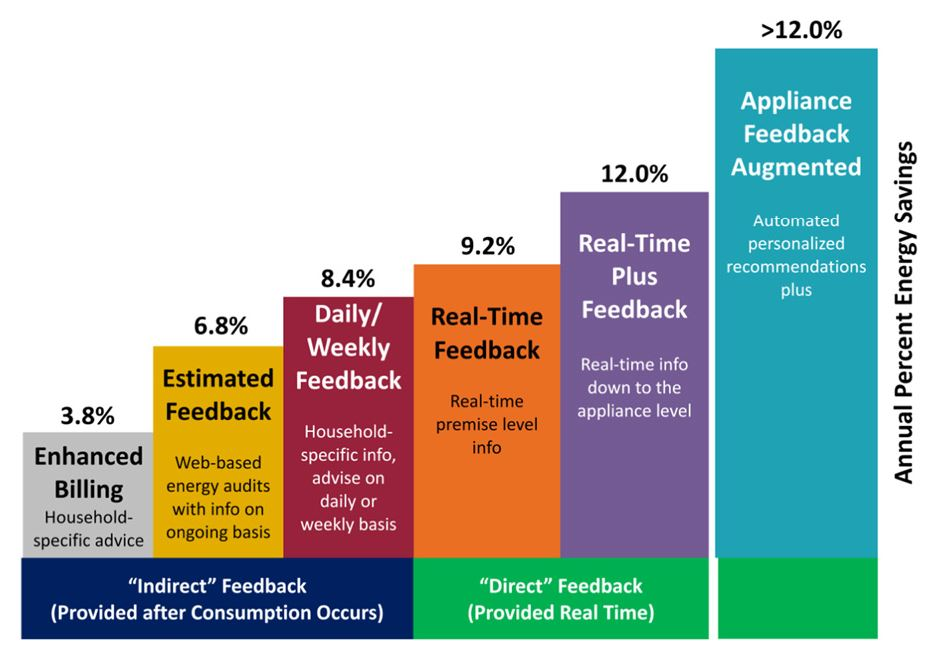
\includegraphics[width=\textwidth]{1_Grafiken/fig1armel.jpg}
	\caption[Einsparungpotentiale nach Ma{\ss}nahme]{Grafik zu Einsparpotetialen je nach getroffener Aufkl"arungsma{\ss}nahme aus \cite{armel2013disaggregation}}
\label{potentiale}
\end{figure}

	Er kann sich oft nicht mit seinem Verbrauch identifizieren, weil dieser intransparent und durch die langen Rechnungsintervalle nicht pr"asent ist. \\
	Damit der Nutzer anf"angt sich selbst zu kontrollieren, muss er begreifen, dass sich sein Verhalten auf seinen Verbrauch auswirkt und er ihn auch durch die gezielte Ver"anderungen seines Handelns senken kann \cite{fischer2008feedback}.\\
	Non-intrusive load monitoring (NILM) bietet nun die Chance dem Nutzer eine regelm"a{\ss}ige, detaillierte R"uckmeldung zu seinem Energiekonsum zu geben, Kolter und Matthew \cite{kolter2011redd} beschreibt NILM als die Aufgabe aus einem, f"ur den gesamten Haushalt messenden Stromz"ahler, R"uckschl"usse "uber die elektrische Last einzelner Ger"ate zu ziehen.
	Ein solches System wird dem Konsumenten helfen, verschwenderische Verhaltensweisen und Ger"ate zu identifizieren ohne den Haushalt mit vielen digitalen Z"ahlern f"ur die individuellen Ger"ate ausr"usten zu m"ussen, wie es derzeit z.B. mit sogenannten \textit{Energiekostenmessger"aten} auf Steckerbasis praktiziert wird.

\subsection{Fragestellung}
\label{Fragestellung}
 	Viele Systeme zur Disagregation oder zu verschiedenen Vorhersage-Aufgaben benutzen Ans"atze des Maschinellen Lernens. Sie ben"otigen annotierte (gelabelte) Trainingsdaten, um robuste Modelle zu erzeugen. Annotieren bedeutet in diesem Zusammenhang, die Daten mit Metadaten wie etwa dem Ger"atezustand zu versehen. Mehr Trainingsdaten f"uhren in der Regel zu besseren Modellen, die Annotation ist allerdings sehr aufw"andig, weil sie manuell erfolgen muss. Der Ansatzpunkt dieser Arbeit ist, das Problem der Disagregation auf ein Ger"at zu reduzieren und so zu vereinfachen. Nun kann man ein robustes Modell mit nur wenigen Trainingsdaten erstellen und mit diesem dann eine gro{\ss}e Menge an Daten schnell annotieren. Diese gelabelten Daten sollen dann wiederum als Trainingsdaten f"ur schwierigere Aufgaben verwendet werden. 
	Aufgabe dieser Bachelorarbeit ist es ein System zu entwickeln, welches in der Lage ist die Zust"ande von ausgew"ahlten Ger"aten in einem disaggregierten Lastgang zu klassifizieren und so eine Segmentierung f"ur diese Ger"ate zu erstellen. Dies beinhaltet sowohl die n"otige Vorverarbeitung der Daten sowie eventuelle nachtr"agliche Formatierungen. Die eigentliche Klassifikation soll mit K"unstlichen Neuronalen Netzen (KNN) stattfinden, dabei sollte eine m"oglichst hohe Akkurarit"at erreicht werden, da Systeme, die mit den resultierenden Daten trainiert werden keine M"oglichkeit haben Fehler, die bereits in den Trainingsdaten sind, zu korrigieren. 
Au{\ss}erdem soll versucht werden aus den klassifizierten Daten wieder einen Lastgang zu erstellen. Dies soll die M"achtigkeit der Segmentierung der Ger"atezust"ande untersuchen und feststellen ob man zuverl"assig den Lastgang des Ger"ats vorhersagen kann, wenn es seine Zustandsfolge im Voraus bekannt gibt. 

\subsection{Weiterer Aufbau}
\label{Weiterer Aufbau}
	Im folgenden Kapitel~\ref{Datensatz} werden die verwendeten, disaggregierten Energiedatens"atze beschrieben. Insbesondere werden die gemessenen Werte und die daraus berechenbaren Werte untersucht. 
	Kapitel~\ref{Vorverarbeitung} gibt zun"achst einen "Uberblick "uber die aktuelle Forschung im Bereich Vorverarbeitung der Daten und Feature-Auswahl, anschlie{\ss}end werden die f"ur diese Arbeit verwendeten Vorverarbeitungsschritte und Features erl"autert.
	In Kapitel~\ref{Klassifizierung} soll schlie{\ss}lich die eigentliche Klassifizierung beschrieben werden, hier werden insbesondere das verwendete Netz und die Trainingsmethoden besprochen. Auch hier wird es einen kurzen "Uberblick "uber die aktuelle Forschung geben.
	In Kapitel~\ref{Generierung} wird die Generierung eines Lastprofils aus dem Zustandsprofil erl"autert. Es wird ein Ansatz aus der aktuellen Forschung beschrieben und auf dieses Problem adaptiert. 
	In Kapitel~\ref{Evaluation} findet die Evaluation statt, hier werden verschiedene Klassifikationsaufgaben ausgef"uhrt und ausgewertet. 
	Am Schluss steht das Fazit in Kapitel~\ref{fazit}, in dem die Ergebnisse zusammengefasst und mit urspr"ungliche Fragestellung verglichen werden.   % Einleitung
%% grundlagen.tex
%% $Id: grundlagen.tex 28 2007-01-18 16:31:32Z bless $
%%

\chapter{Grundlagen}
\label{ch:Grundlagen}
%% ==============================
Die Grundlagen müssen soweit beschrieben
werden, dass ein Leser das Problem und
die Problemlösung  versteht.Um nicht zuviel 
zu beschreiben, kann man das auch erst gegen 
Ende der Arbeit schreiben.

Bla fasel\ldots

%% ==============================
\section{Abschnitt 1}
%% ==============================
\label{ch:Grundlagen:sec:Abschnitt1}

Bla fasel\ldots

%% ==============================
\section{Abschnitt 2}
%% ==============================
\label{ch:Grundlagen:sec:Abschnitt2}

Bla fasel\ldots

%% ==============================
\section{Verwandte Arbeiten}
%% ==============================
\label{ch:Grundlagen:sec:RelatedWork}
Hier kommt "`Related Work"' rein.
Eine Literaturrecherche sollte so vollständig wie möglich sein,
relevante Ansätze müssen beschrieben werden und es sollte deutlich 
gemacht werden, wo diese Ansätze Defizite aufweisen oder nicht
anwendbar sind, z.\,B. weil sie von anderen Umgebungen oder 
Voraussetzungen ausgehen.


Bla fasel\ldots

%%% Local Variables: 
%%% mode: latex
%%% TeX-master: "diplarb"
%%% End: 
  % Grundlagen
%% analyse.tex
%% $Id: analyse.tex 28 2007-01-18 16:31:32Z bless $

\chapter{Analyse}
\label{ch:Analyse}
%% ==============================
In diesem Kapitel sollten zun�chst das zu l�sende Problem
sowie die Anforderungen und die Randbedingungen 
einer L�sung\index{L�sung} beschrieben werden (also nochmal
eine pr�zisierte Aufgabenstellung\index{Aufgabenstellung}).

Dann folgt �blicherweise ein �berblick �ber bereits existierende
L�sungen bzw. Ans�tze, die meistens andere Voraussetzungen bzw.
Randbedingungen annehmen.

Bla fasel\ldots

%% ==============================
\section{Anforderungen}
%% ==============================
\label{ch:Analyse:sec:Anforderungen}
Anforderungen und Randbedingungen\index{Randbedingungen} \ldots

%% ==============================
\section{Existierende L�sungsans�tze}
%% ==============================
\label{ch:Analyse:sec:RelatedWork}

Hier kommt eine ausf�hrliche Diskussion
von "`Related Work"'.

Bla fasel\ldots

%% ==============================
\section{Weiterer Abschnitt}
%% ==============================
\label{ch:Analyse:sec:Abschnitt}

Bla fasel\ldots Abbildung~\ref{fig:test} auf S.~\pageref{fig:test} sollte man
sich mal anschauen.

Lorem ipsum dolor sit amet, consetetur sadipscing elitr, sed diam nonumy eirmod tempor invidunt ut labore et dolore magna aliquyam erat, sed diam voluptua.
At vero eos et accusam et justo duo dolores et ea rebum. \cite{TB2000}
Stet clita kasd gubergren, no sea takimata sanctus est Lorem ipsum dolor sit amet. Lorem ipsum dolor sit amet, consetetur sadipscing elitr, sed diam nonumy eirmod tempor invidunt ut labore et dolore magna aliquyam erat, sed diam voluptua. At vero eos et accusam et justo duo dolores et ea rebum. Stet clita kasd gubergren, no sea takimata sanctus est Lorem ipsum dolor sit amet. Lorem ipsum dolor sit amet, consetetur sadipscing elitr, sed diam nonumy eirmod tempor invidunt ut labore et dolore magna aliquyam erat, sed diam voluptua. At vero eos et accusam et justo duo dolores et ea rebum. Stet clita kasd gubergren, no sea takimata sanctus est Lorem ipsum dolor sit amet. 

Duis autem vel eum iriure dolor in hendrerit in vulputate velit esse molestie consequat, vel illum dolore eu feugiat nulla facilisis at vero eros et accumsan et iusto odio dignissim qui blandit praesent luptatum zzril delenit augue duis dolore te feugait nulla facilisi.
$$ u(x,t)= 8 \frac{k_{1}^{2}e^{\alpha_{1}} + k_{2}^{2}e^{\alpha_{2}} + (k_{1}-k_{2})^{2}e^{(\alpha_{1}+ \alpha_{2})} \left[2 + \frac{1}{(k_{1} + k_{2})^{2}} ( k_{1}^{2}e^{\alpha_{1}} + k_{2}^{2}e^{\alpha_{2}}) \right]}{\left[1+e^{\alpha_{1}} + e^{\alpha_{2}} + \left(\frac{k_{1} - k_{2}}{k_{1}+k_{2}} \right)^{2} e^{\alpha_{1}+ \alpha_{2}} \right]^{2}} $$ Lorem ipsum dolor sit amet, consectetuer adipiscing elit, sed diam nonummy nibh euismod tincidunt ut laoreet dolore magna aliquam erat volutpat.

Ut wisi enim ad minim veniam, quis nostrud exerci tation ullamcorper suscipit lobortis nisl ut aliquip ex ea commodo consequat. Duis autem vel eum iriure dolor in hendrerit in vulputate velit esse molestie consequat, vel illum dolore eu feugiat nulla facilisis at vero eros et accumsan et iusto odio dignissim qui blandit praesent luptatum zzril delenit augue duis dolore te feugait nulla facilisi. 

Nam liber tempor cum soluta nobis eleifend option congue nihil imperdiet doming id quod mazim placerat facer possim assum. Lorem ipsum dolor sit amet, consectetuer adipiscing elit, sed diam nonummy nibh euismod tincidunt ut laoreet dolore magna aliquam erat volutpat. Ut wisi enim ad minim veniam, quis nostrud exerci tation ullamcorper suscipit lobortis nisl ut aliquip ex ea commodo consequat. \cite{TB98,JSAC96,qosr}

Duis autem vel eum iriure dolor in hendrerit in vulputate velit esse molestie consequat, vel illum dolore eu feugiat nulla facilisis. 

At vero eos et accusam et justo duo dolores et ea rebum. Stet clita kasd gubergren, no sea takimata sanctus est Lorem ipsum dolor sit amet. Lorem ipsum dolor sit amet, consetetur sadipscing elitr, sed diam nonumy eirmod tempor invidunt ut labore et dolore magna aliquyam erat, sed diam voluptua. At vero eos et accusam et justo duo dolores et ea rebum. Stet clita kasd gubergren, no sea takimata sanctus est Lorem ipsum dolor sit amet. Lorem ipsum dolor sit amet, consetetur sadipscing elitr, At accusam aliquyam diam diam dolore dolores duo eirmod eos erat, et nonumy sed tempor et et invidunt justo labore Stet clita ea et gubergren, kasd magna no rebum. sanctus sea sed takimata ut vero voluptua. est Lorem ipsum dolor sit amet. Lorem ipsum dolor sit amet, consetetur sadipscing elitr, sed diam nonumy eirmod tempor invidunt ut labore et dolore magna aliquyam erat. 

Consetetur sadipscing elitr, sed diam nonumy eirmod tempor invidunt ut labore et dolore magna aliquyam erat, sed diam voluptua. At vero eos et accusam et justo duo dolores et ea rebum. Stet clita kasd gubergren, no sea takimata sanctus est Lorem ipsum dolor sit amet. Lorem ipsum dolor sit amet, consetetur sadipscing elitr, sed diam nonumy eirmod tempor invidunt ut labore et dolore magna aliquyam erat, sed diam voluptua. At vero eos et accusam et justo duo dolores et ea rebum. Stet clita kasd gubergren, no sea takimata sanctus est Lorem ipsum dolor sit amet. Lorem ipsum dolor sit amet, consetetur sadipscing elitr, sed diam nonumy eirmod tempor invidunt ut labore et dolore magna aliquyam erat, sed diam voluptua. At vero eos et accusam et justo duo dolores et ea rebum. Stet clita kasd gubergren, no sea takimata sanctus. 

Lorem ipsum dolor sit amet, consetetur sadipscing elitr, sed diam nonumy eirmod tempor invidunt ut labore et dolore magna aliquyam erat, sed diam voluptua. At vero eos et accusam et justo duo dolores et ea rebum. Stet clita kasd gubergren, no sea takimata sanctus est Lorem ipsum dolor sit amet. Lorem ipsum dolor sit amet, consetetur sadipscing elitr, sed diam nonumy eirmod tempor invidunt ut labore et dolore magna aliquyam erat, sed diam voluptua. At vero eos et accusam et justo duo dolores et ea rebum. Stet clita kasd gubergren, no sea takimata sanctus est Lorem ipsum dolor sit amet. Lorem ipsum dolor sit amet, consetetur sadipscing elitr, sed diam nonumy eirmod tempor invidunt ut labore et dolore magna aliquyam erat, sed diam voluptua. At vero eos et accusam et justo duo dolores et ea rebum. Stet clita kasd gubergren, no sea takimata sanctus est Lorem ipsum dolor sit amet. 

Duis autem vel eum iriure dolor in hendrerit in vulputate velit esse molestie consequat, vel illum dolore eu feugiat nulla facilisis at vero eros et accumsan et iusto odio dignissim qui blandit praesent luptatum zzril delenit augue duis dolore te feugait nulla facilisi. Lorem ipsum dolor sit amet, consectetuer adipiscing elit, sed diam nonummy nibh euismod tincidunt ut laoreet dolore magna aliquam erat volutpat. 

Ut wisi enim ad minim veniam, quis nostrud exerci tation ullamcorper suscipit lobortis nisl ut aliquip ex ea commodo consequat. Duis autem vel eum iriure dolor in hendrerit in vulputate velit esse molestie consequat, vel illum dolore eu feugiat nulla facilisis at vero eros et accumsan et iusto odio dignissim qui blandit praesent luptatum zzril delenit augue duis dolore te feugait nulla facilisi. 

Blindtext Blindtext Blindtext\index{Blindtext} Blindtext Blindtext Blindtext Blindtext

\begin{figure}[!htbp]
  \centering
  \fbox{\parbox{0.8\textwidth}{
  Abbildungen sollten m�glichst als EPS (Encapsulated Postscript) 
  bzw. PDF eingebunden werden.
  Zur Erzeugung sauberer EPS-Dateien empfiehlt sich das Tool \texttt{ps2eps}
  zur Nachbearbeitung von Postscript-Dateien. Mit \texttt{epstopdf} kann
  dann eine PDF-Datei zum Einbinden erzeugt werden.}}
  \caption{Testabbildung}
  \label{fig:test}
\end{figure}

Lorem ipsum dolor sit amet, consetetur sadipscing elitr, sed diam nonumy eirmod tempor invidunt ut labore et dolore magna aliquyam erat, sed diam voluptua. At vero eos et accusam et justo duo dolores et ea rebum. Stet clita kasd gubergren, no sea takimata sanctus est Lorem ipsum dolor sit amet. Lorem ipsum dolor sit amet, consetetur sadipscing elitr, sed diam nonumy eirmod tempor invidunt ut labore et dolore magna aliquyam erat, sed diam voluptua. At vero eos et accusam et justo duo dolores et ea rebum. Stet clita kasd gubergren, no sea takimata sanctus est Lorem ipsum dolor sit amet. Lorem ipsum dolor sit amet, consetetur sadipscing elitr, sed diam nonumy eirmod tempor invidunt ut labore et dolore magna aliquyam erat, sed diam voluptua. At vero eos et accusam et justo duo dolores et ea rebum. Stet clita kasd gubergren, no sea takimata sanctus est Lorem ipsum dolor sit amet. 

Duis autem vel eum iriure dolor in hendrerit in vulputate velit esse molestie consequat, vel illum dolore eu feugiat nulla facilisis at vero eros et accumsan et iusto odio dignissim qui blandit praesent luptatum zzril delenit augue duis dolore te feugait nulla facilisi. Lorem ipsum dolor sit amet, consectetuer adipiscing elit, sed diam nonummy nibh euismod tincidunt ut laoreet dolore magna aliquam erat volutpat. 

Ut wisi enim ad minim veniam, quis nostrud exerci tation ullamcorper suscipit lobortis nisl ut aliquip ex ea commodo consequat. Duis autem vel eum iriure dolor in hendrerit in vulputate velit esse molestie consequat, vel illum dolore eu feugiat nulla facilisis at vero eros et accumsan et iusto odio dignissim qui blandit praesent luptatum zzril delenit augue duis dolore te feugait nulla facilisi. 

Nam liber tempor cum soluta nobis eleifend option congue nihil imperdiet doming id quod mazim placerat facer possim assum. Lorem ipsum dolor sit amet, consectetuer adipiscing elit, sed diam nonummy nibh euismod tincidunt ut laoreet dolore magna aliquam erat volutpat. Ut wisi enim ad minim veniam, quis nostrud exerci tation ullamcorper suscipit lobortis nisl ut aliquip ex ea commodo consequat. 

Duis autem vel eum iriure dolor in hendrerit in vulputate velit esse molestie consequat, vel illum dolore eu feugiat nulla facilisis. 

At vero eos et accusam et justo duo dolores et ea rebum. Stet clita kasd gubergren, no sea takimata sanctus est Lorem ipsum dolor sit amet. Lorem ipsum dolor sit amet, consetetur sadipscing elitr, sed diam nonumy eirmod tempor invidunt ut labore et dolore magna aliquyam erat, sed diam voluptua. At vero eos et accusam et justo duo dolores et ea rebum. Stet clita kasd gubergren, no sea takimata sanctus est Lorem ipsum dolor sit amet. Lorem ipsum dolor sit amet, consetetur sadipscing elitr, At accusam aliquyam diam diam dolore dolores duo eirmod eos erat, et nonumy sed tempor et et invidunt justo labore Stet clita ea et gubergren, kasd magna no rebum. sanctus sea sed takimata ut vero voluptua. est Lorem ipsum dolor sit amet. Lorem ipsum dolor sit amet, consetetur sadipscing elitr, sed diam nonumy eirmod tempor invidunt ut labore et dolore magna aliquyam erat. 

Consetetur sadipscing elitr, sed diam nonumy eirmod tempor invidunt ut labore et dolore magna aliquyam erat, sed diam voluptua. At vero eos et accusam et justo duo dolores et ea rebum. Stet clita kasd gubergren, no sea takimata sanctus est Lorem ipsum dolor sit amet. Lorem ipsum dolor sit amet, consetetur sadipscing elitr, sed diam nonumy eirmod tempor invidunt ut labore et dolore magna aliquyam erat, sed diam voluptua. At vero eos et accusam et justo duo dolores et ea rebum. Stet clita kasd gubergren, no sea takimata sanctus est Lorem ipsum dolor sit amet. Lorem ipsum dolor sit amet, consetetur sadipscing elitr, sed diam nonumy eirmod tempor invidunt ut labore et dolore magna aliquyam erat, sed diam voluptua. At vero eos et accusam et justo duo dolores et ea rebum. Stet clita kasd gubergren, no sea takimata sanctus. 

Lorem ipsum dolor sit amet, consetetur sadipscing elitr, sed diam nonumy eirmod tempor invidunt ut labore et dolore magna aliquyam erat, sed diam voluptua. At vero eos et accusam et justo duo dolores et ea rebum. Stet clita kasd gubergren, no sea takimata sanctus est Lorem ipsum dolor sit amet. Lorem ipsum dolor sit amet, consetetur sadipscing elitr, sed diam nonumy eirmod tempor invidunt ut labore et dolore magna aliquyam erat, sed diam voluptua. At vero eos et accusam et justo duo dolores et ea rebum. Stet clita kasd gubergren, no sea takimata sanctus est Lorem ipsum dolor sit amet. Lorem ipsum dolor sit amet, consetetur sadipscing elitr, sed diam nonumy eirmod tempor invidunt ut labore et dolore magna aliquyam erat, sed diam voluptua. At vero eos et accusam et justo duo dolores et ea rebum. Stet clita kasd gubergren, no sea takimata sanctus est Lorem ipsum dolor sit amet. 

Duis autem vel eum iriure dolor in hendrerit in vulputate velit esse molestie consequat, vel illum dolore eu feugiat nulla facilisis at vero eros et accumsan et iusto odio dignissim qui blandit praesent luptatum zzril delenit augue duis dolore te feugait nulla facilisi. Lorem ipsum dolor sit amet, consectetuer adipiscing elit, sed diam nonummy nibh euismod tincidunt ut laoreet dolore magna aliquam erat volutpat. 

Ut wisi enim ad minim veniam, quis nostrud exerci tation ullamcorper suscipit lobortis nisl ut aliquip ex ea commodo consequat. Duis autem vel eum iriure dolor in hendrerit in vulputate velit esse molestie consequat, vel illum dolore eu feugiat nulla facilisis at vero eros et accumsan et iusto odio dignissim qui blandit praesent luptatum zzril delenit augue duis dolore te feugait nulla facilisi. 

%% ==============================
\section{Zusammenfassung}
%% ==============================
\label{ch:Analyse:sec:zusammenfassung}

Am Ende sollten ggf. die wichtigsten Ergebnisse nochmal in \emph{einem}
kurzen Absatz zusammengefasst werden.

%%% Local Variables: 
%%% mode: latex
%%% TeX-master: "diplarb"
%%% End: 
     % Analyse
%% entwurf.tex
%% $Id: entwurf.tex 28 2007-01-18 16:31:32Z bless $
%%

\chapter{Entwurf}
\label{ch:Entwurf}
%% ==============================
In diesem Kapitel erfolgt die ausf�hrliche Beschreibung des eigenen
L�sungsansatzes. Dabei sollten L�sungsalternativen diskutiert und
Entwurfsentscheidungen dargelegt werden.


Bla fasel\ldots

%% ==============================
\section{Abschnitt 1}
%% ==============================
\label{ch:Entwurf:sec:Abschnitt1}

Bla fasel\ldots

%% ==============================
\section{Abschnitt 2}
%% ==============================
\label{ch:Entwurf:sec:Abschnitt2}

Bla fasel\ldots

Blindtext Blindtext Blindtext Blindtext Blindtext Blindtext Blindtext
Blindtext Blindtext Blindtext Blindtext Blindtext Blindtext Blindtext
Blindtext Blindtext Blindtext Blindtext Blindtext Blindtext Blindtext
Blindtext Blindtext Blindtext Blindtext Blindtext Blindtext Blindtext
Blindtext Blindtext Blindtext Blindtext Blindtext Blindtext Blindtext
Blindtext Blindtext Blindtext Blindtext Blindtext Blindtext Blindtext
Blindtext Blindtext Blindtext Blindtext Blindtext Blindtext Blindtext
Blindtext Blindtext Blindtext Blindtext Blindtext Blindtext Blindtext
Blindtext Blindtext Blindtext Blindtext Blindtext Blindtext Blindtext
Blindtext Blindtext Blindtext Blindtext Blindtext Blindtext Blindtext
Blindtext Blindtext Blindtext Blindtext Blindtext Blindtext Blindtext
Blindtext Blindtext Blindtext Blindtext Blindtext Blindtext Blindtext
Blindtext Blindtext Blindtext Blindtext Blindtext Blindtext Blindtext
Blindtext Blindtext Blindtext Blindtext Blindtext Blindtext Blindtext
Blindtext Blindtext Blindtext Blindtext Blindtext Blindtext Blindtext
Blindtext Blindtext Blindtext Blindtext Blindtext Blindtext Blindtext
Blindtext Blindtext Blindtext Blindtext Blindtext Blindtext Blindtext

Blindtext Blindtext Blindtext Blindtext Blindtext Blindtext Blindtext
Blindtext Blindtext Blindtext Blindtext Blindtext Blindtext Blindtext
Blindtext Blindtext Blindtext Blindtext Blindtext Blindtext Blindtext
Blindtext Blindtext Blindtext Blindtext Blindtext Blindtext Blindtext
Blindtext Blindtext Blindtext Blindtext Blindtext Blindtext Blindtext
Blindtext Blindtext Blindtext Blindtext Blindtext Blindtext Blindtext
Blindtext Blindtext Blindtext Blindtext Blindtext Blindtext Blindtext
Blindtext Blindtext Blindtext Blindtext Blindtext Blindtext Blindtext
Blindtext Blindtext Blindtext Blindtext Blindtext Blindtext Blindtext
Blindtext Blindtext Blindtext Blindtext Blindtext Blindtext Blindtext
Blindtext Blindtext Blindtext Blindtext Blindtext Blindtext Blindtext
Blindtext Blindtext Blindtext Blindtext Blindtext Blindtext Blindtext
Blindtext Blindtext Blindtext Blindtext Blindtext Blindtext Blindtext
Blindtext Blindtext Blindtext Blindtext Blindtext Blindtext Blindtext
Blindtext Blindtext Blindtext Blindtext Blindtext Blindtext Blindtext
Blindtext Blindtext Blindtext Blindtext Blindtext Blindtext Blindtext
Blindtext Blindtext Blindtext Blindtext Blindtext Blindtext Blindtext
Blindtext Blindtext Blindtext Blindtext Blindtext Blindtext Blindtext
Blindtext Blindtext Blindtext Blindtext Blindtext Blindtext Blindtext
Blindtext Blindtext Blindtext Blindtext Blindtext Blindtext Blindtext

Blindtext Blindtext Blindtext Blindtext Blindtext Blindtext Blindtext
Blindtext Blindtext Blindtext Blindtext Blindtext Blindtext Blindtext
Blindtext Blindtext Blindtext Blindtext Blindtext Blindtext Blindtext
Blindtext Blindtext Blindtext Blindtext Blindtext Blindtext Blindtext
Blindtext Blindtext Blindtext Blindtext Blindtext Blindtext Blindtext
Blindtext Blindtext Blindtext Blindtext Blindtext Blindtext Blindtext
Blindtext Blindtext Blindtext Blindtext Blindtext Blindtext Blindtext
Blindtext Blindtext Blindtext Blindtext Blindtext Blindtext Blindtext
Blindtext Blindtext Blindtext Blindtext Blindtext Blindtext Blindtext
Blindtext Blindtext Blindtext Blindtext Blindtext Blindtext Blindtext
Blindtext Blindtext Blindtext Blindtext Blindtext Blindtext Blindtext
Blindtext Blindtext Blindtext Blindtext Blindtext Blindtext Blindtext
Blindtext Blindtext Blindtext Blindtext Blindtext Blindtext Blindtext
Blindtext Blindtext Blindtext Blindtext Blindtext Blindtext Blindtext
Blindtext Blindtext Blindtext Blindtext Blindtext Blindtext Blindtext

Blindtext Blindtext Blindtext Blindtext Blindtext Blindtext Blindtext
Blindtext Blindtext Blindtext Blindtext Blindtext Blindtext Blindtext
Blindtext Blindtext Blindtext Blindtext Blindtext Blindtext Blindtext
Blindtext Blindtext Blindtext Blindtext Blindtext Blindtext Blindtext
Blindtext Blindtext Blindtext Blindtext Blindtext Blindtext Blindtext
Blindtext Blindtext Blindtext Blindtext Blindtext Blindtext Blindtext
Blindtext Blindtext Blindtext Blindtext Blindtext Blindtext Blindtext
Blindtext Blindtext Blindtext Blindtext Blindtext Blindtext Blindtext
Blindtext Blindtext Blindtext Blindtext Blindtext Blindtext Blindtext
Blindtext Blindtext Blindtext Blindtext Blindtext Blindtext Blindtext
Blindtext Blindtext Blindtext Blindtext Blindtext Blindtext Blindtext
Blindtext Blindtext Blindtext Blindtext Blindtext Blindtext Blindtext
Blindtext Blindtext Blindtext Blindtext Blindtext Blindtext Blindtext
Blindtext Blindtext Blindtext Blindtext Blindtext Blindtext Blindtext
Blindtext Blindtext Blindtext Blindtext Blindtext Blindtext Blindtext
Blindtext Blindtext Blindtext Blindtext Blindtext Blindtext Blindtext

Blindtext Blindtext Blindtext Blindtext Blindtext Blindtext Blindtext
Blindtext Blindtext Blindtext Blindtext Blindtext Blindtext Blindtext
Blindtext Blindtext Blindtext Blindtext Blindtext Blindtext Blindtext
Blindtext Blindtext Blindtext Blindtext Blindtext Blindtext Blindtext
Blindtext Blindtext Blindtext Blindtext Blindtext Blindtext Blindtext
Blindtext Blindtext Blindtext Blindtext Blindtext Blindtext Blindtext
Blindtext Blindtext Blindtext Blindtext Blindtext Blindtext Blindtext
Blindtext Blindtext Blindtext Blindtext Blindtext Blindtext Blindtext
Blindtext Blindtext Blindtext Blindtext Blindtext Blindtext Blindtext
Blindtext Blindtext Blindtext Blindtext Blindtext Blindtext Blindtext
Blindtext Blindtext Blindtext Blindtext Blindtext Blindtext Blindtext
Blindtext Blindtext Blindtext Blindtext Blindtext Blindtext Blindtext
Blindtext Blindtext Blindtext Blindtext Blindtext Blindtext Blindtext

%% ==============================
\section{Zusammenfassung}
%% ==============================
\label{ch:Entwurf:sec:zusammenfassung}

Am Ende sollten ggf. die wichtigsten Ergebnisse nochmal in \emph{einem}
kurzen Absatz zusammengefasst werden.

%%% Local Variables: 
%%% mode: latex
%%% TeX-master: "diplarb"
%%% End: 
     % Entwurf
%% implemen.tex
%% $Id: implemen.tex 4 2005-10-10 20:51:21Z bless $
%%

\chapter{Implementierung}
\label{ch:Implementierung}
%% ==============================
Bla fasel\ldots

%% ==============================
\section{Abschnitt 1}
%% ==============================
\label{ch:Implementierung:sec:Abschnitt1}

Bla fasel\ldots

%% ==============================
\section{Abschnitt 2}
%% ==============================
\label{ch:Implementierung:sec:Abschnitt2}

Bla fasel\ldots

%%% Local Variables: 
%%% mode: latex
%%% TeX-master: "diplarb"
%%% End: 
    % Implementierung
%% eval.tex
%% $Id: eval.tex 5 2005-10-10 20:55:48Z bless $

\chapter{Evaluierung}
\label{ch:Evaluierung}
%% ==============================
Hier kommt der Nachweis, dass das in Kapitel~\ref{ch:Entwurf}
entworfene Konzept auch funktioniert. Leistungsmessungen einer
Implementierung werden auch immer gerne gesehen.

Bla fasel\ldots

%% ==============================
\section{Abschnitt 1}
%% ==============================
\label{ch:Evaluierung:sec:Abschnitt1}

Bla fasel\ldots

%% ==============================
\section{Abschnitt 2}
%% ==============================
\label{ch:Evaluierung:sec:Abschnitt2}

Bla fasel\ldots

%% ==============================
\section{Zusammenfassung}
%% ==============================
\label{ch:Evaluierung:sec:zusammenfassung}

Am Ende sollten ggf. die wichtigsten Ergebnisse nochmal in \emph{einem}
kurzen Absatz zusammengefasst werden.

%%% Local Variables: 
%%% mode: latex
%%% TeX-master: "diplarb"
%%% End: 
        % Evaluierung
%% zusammenf.tex
%% $Id: zusammenf.tex 4 2005-10-10 20:51:21Z bless $
%%

\chapter{Zusammenfassung und Ausblick}
\label{ch:Zusammenfassung}
%% ==============================
Bla fasel\ldots

(Keine Untergliederung mehr!)

%%% Local Variables: 
%%% mode: latex
%%% TeX-master: "diplarb"
%%% End: 
   % Zusammenfassung und Ausblick

%% ++++++++++++++++++++++++++++++++++++++++++
%% Anhang
%% ++++++++++++++++++++++++++++++++++++++++++

\appendix
%\include{anhang_a}
%\include{anhang_b}

%% ++++++++++++++++++++++++++++++++++++++++++
%% Literatur
%% ++++++++++++++++++++++++++++++++++++++++++
%  mit dem Befehl \nocite werden auch nicht 
%  zitierte Referenzen abgedruckt
\cleardoublepage
\phantomsection
\addcontentsline{toc}{chapter}{\bibname}
%%
\nocite{*} % nur angeben, wenn auch nicht im Text zitierte Quellen 
           % erscheinen sollen
\bibliographystyle{itmabbrv} % mit abgek�rzten Vornamen der Autoren
%\bibliographystyle{gerplain} % abbrvnat unsrtnat
% spezielle Zitierstile: Labels mit vier Buchstaben und Jahreszahl
%\bibliographystyle{itmalpha}  % ausgeschriebene Vornamen der Autoren
\bibliography{diplarb}
%% ++++++++++++++++++++++++++++++++++++++++++
%% Index
%% ++++++++++++++++++++++++++++++++++++++++++
\ifnotdraft{
\cleardoublepage
\phantomsection
\printindex            % Index, Stichwortverzeichnis
}
\end{document}
%% end of file
